\documentclass[a4paper,twoside,10pt]{article}
\linespread{1}                     % For line spacing
\usepackage{amssymb}                 % For AMS symbol
\usepackage{amsmath,amsthm,latexsym}                 % This is useful for the matrix $\begin{bmatrix} a & b\\ 0 & c\end{bmatrix}$
\usepackage{verbatim}                % For comments in paragraph
\usepackage{graphicx}
\usepackage{epstopdf}
\usepackage{epsfig}              % For imbeding graph
\usepackage{color}                  % Color for the text
\usepackage[normal]{caption2}
\usepackage[utf8]{inputenc}
\usepackage[english]{babel}
\usepackage{multicol}
\setlength{\columnsep}{0.8cm}
\usepackage{makeidx}
\usepackage[normal]{subfigure}
\usepackage{url}
\usepackage{lineno}
\usepackage{hyperref}
\usepackage{mathtools}
\usepackage{plain}
%%%%%%%%%%%%%
\textheight23cm%25.0cm
\textwidth16.3cm
\oddsidemargin-0.1cm
\evensidemargin0.1cm
%\topmargin-1cm
\headsep.3cm
%\usepackage{pstricks}
\usepackage{fancyhdr}
\pagestyle{fancy}
\fancyhf{}% Clear header/footer
\fancyhead[OC]{Journal of Nepal Mathematical Society (JNMS), Vol. --, Issue -- (202--); S. Thakuri, B.H Subedi}%Author on Odd page, Centred
\fancyhead[EC]{Applications of Galois Theory}% Title on Even page, Centred
\fancyfoot[C]{\thepage}%

% Added package by the author-------------------------------------------------------------------------------------------------
\usepackage{tikz, pgfplots}
\usepgflibrary{shadings}
\usetikzlibrary{positioning, shapes.geometric}
\pgfplotsset{compat=1.18}

\theoremstyle{plain}
\newtheorem{theorem}{Theorem}[section]
\newtheorem{lemma}[theorem]{Lemma}
\newtheorem{corollary}[theorem]{Corollary}
\newtheorem{algorithm}[theorem]{Algorithm}

\theoremstyle{definition}
\newtheorem{definition}[theorem]{Definition}
\newtheorem{example}[theorem]{Example}
\newtheorem{remark}[theorem]{Remark}

%---------------------------------------------------------------------------------------------------------------------------------------------------------------------------------
\begin{document}
\linenumbers
{\Large
\begin{center}
\bf{\LARGE Applications of Galois Theory}
\end{center}}
\begin{center}
Sandesh Thakuri$^{1}$, Bishnu Hari Subedi$^{2}$
\end{center}

\begin{center}
{\footnotesize
$^{1,2}$Central Department of Mathematics, Tribhuvan University, Kirtipur, Kathmandu, Nepal \\[1mm]
Correspondence to: Sandesh Thakuri, Email: sandeshthakuri111@gmail.com
}
\end{center}

\noindent
\textbf{Abstract:} {\it This paper gives an insight to the Galois theory and discusses its applications in both pure and applied mathematics. First the Fundamental theorem of Galois theory is applied to compute the Galois groups of polynomials and to prove the non-existence of a formula for solving a polynomial equations in rationals having degree \(n \geq 5\). Then the Galois fields which are finite fields are applied to the error-correcting codes and cryptography in computer science. There are no general rules to compute the Galois groups of polynomials of degree more than four. Two new examples of Galois groups of polynomials of degree greater than four are introduced and the concept of Galois group of a single variable polynomial is extended to the Galois group of a multi-variable polynomial.}\\\\
\textbf{Keywords:} Fundamental theorem, Galois group, Galois field, Error-correcting codes, Cryptography

\section{Introduction}
The foundation of Galois theory was laid by the French mathematician \textit{Évariste Galois}(1811-1832) by determining the necessary and sufficient condition for solving a polynomial equation by radicals \cite{galois}. Galois theory has evolved a lot from then and has found its applications in wide range of fields from pure mathematics especially in abstract algebra, algebraic number theory to algebraic geometry to applied mathematics. This paper is limited to its applications in abstract algebra and in computer science. \\[2mm]
Modern Galois theory is a theory of field extension which is a vast theory. The core-part of the Galois theory is the ``Fundamental theorem of Galois theory'' \cite {hunger}. The Fundamental theorem links a Galois extension to its Galois group. Let \(F\) be an extension field of a field \(K\). The group of all automorphisms of \(F\) that fixes \(K\) is called the Galois group of \(F\) over \(K\) and it is denoted by \(Aut_K^F\) \cite{hunger}. The extension field \(F\) of \(K\) is said to be a Galois extension of \(K\) or Galois over K if the fixed field of the Galois group \(Aut_k^F\) is \(K\) itself \cite{hunger}.

\begin{theorem} \cite{hunger} [\textbf{The Fundamental Theorem}]
  If \(F\) is a finite dimensional Galois extension of \(K\), then there is a one-to-one correspondence between the set of all intermediate fields of \(F\) over \(K\) and the set of subgroups of the Galois group \(Aut_K^F\) such that:
  \begin{enumerate}
  \item[i)] the relative dimension of two intermediate fields is equal to the relative index of the corresponding subgroups. In particular \(Aut_K^F\) has order \([F:K]\);
  \item[ii)] \(F\) is Galois over every intermediate field \(E\), but \(E\) is Galois over \(K\) if and only if the corresponding subgroup \(E'= Aut_E^F\) is normal in \(G=Aut_K^F\). In this case \(G/E'\) is isomorphic to the Galois group \(Aut_K^E\) of \(E\) over \(K\).
  \end{enumerate}
\end{theorem}
\vspace{2mm}
\noindent
A field \(E\) such that \(K \subset E \subset F\) is said to be an intermediate field of \(F\) over \(K\) \cite{hunger}. The index of a subgroup \(H\) of a group \(G\) is the ration of order of \(G\) over \(H\) \cite{hunger}.\\[3mm]

\noindent
The Fundamental theorem links field theory to group theory. This allows us to use the tools of group theory to solve the problems of field theory. Solving a polynomial equation is a problem of field theory. We can use the insights of group theory to solve this problem of field theory which is discussed in some detail in the coming section.
\clearpage

Also, the Fundamental theorem gives some insights of the structure of a field extension. The structure of a field as an extension field over some field is mirrored in the structure of its Galois group which is a group of automorphisms but these automorphisms are the symmetries of the field. \textit{So, the structure of field extension is equals to its own symmetry}. And the structure of a field is a complicated thing; specially if it is infinite. But the structure of a group is rather a simple thing; especially if it is finite. So the Galois theory has fairly simplified the complicated thing in a very insightful and beautiful way. So, Galois theory gives a new sights of study of fields which is study of fields via study of its automorphisms.
\begin{figure}[h]
  \centering
  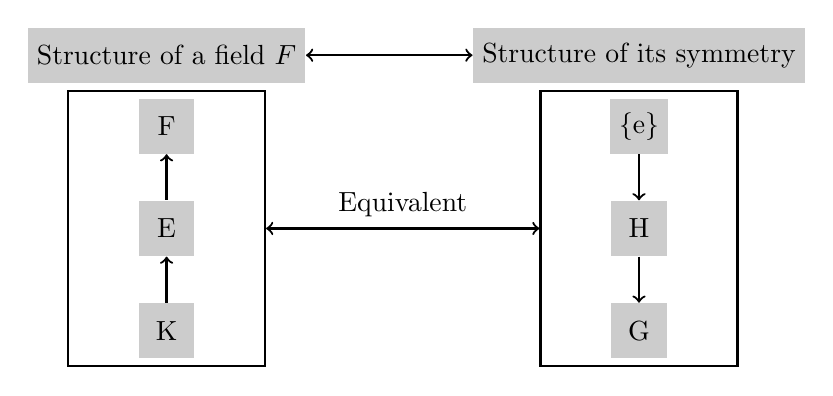
\begin{tikzpicture}

    \node[rectangle, thick, draw,
    minimum height=3.5cm,
    minimum width=2.5cm] (rec) at (0,0) {};

    \node[rectangle, thick, draw,
    minimum height=3.5cm,
    minimum width=2.5cm] (rec2) at (6,0) {};


    \node[minimum width=7mm,
      minimum height=7mm,
      fill=gray!40,
      ] (ss) at (0,2.2) {Structure of a field \(F\)};

      \node[minimum width=7mm,
      minimum height=7mm,
      fill=gray!40,
      ] (ss2) at (6,2.2) {Structure of its symmetry};

      \draw[<->, thick] (ss)--(ss2);
      \draw[<->, thick] (rec)--(rec2);

      \node[minimum width=7mm,
      minimum height=7mm,
      fill=gray!40] (f) at (0,1.3) {F};

      \node[minimum width=7mm,
      minimum height=7mm,
      fill=gray!40,
      below of=f, yshift=-3mm] (e) {E};

      \node[right of=e,
      xshift=20mm, yshift=3mm] (txt) {Equivalent};


      \node[minimum width=7mm,
      minimum height=7mm,
      fill=gray!40,
      below of=e, yshift=-3mm] (k) {K};

      \draw[<-,thick] (f)--(e);
      \draw[<-,thick] (e)--(k);

      \node[right of=f,
      xshift=5cm,
      minimum width=7mm,
      minimum height=7mm,
      fill=gray!40,
      ] (i) {\{e\}};

      \node[minimum width=7mm,
      minimum height=7mm,
      fill=gray!40,
      below of=i, yshift=-3mm] (h) { H};

      \node[
      minimum width=7mm,
      minimum height=7mm,
      fill=gray!40,
      below of=h, yshift=-3mm] (g) {G};

      \draw[->, thick] (i)--(h);
      \draw[->, thick] (h)--(g);
    \end{tikzpicture}
    \caption{\footnotesize Equivalency}
  \end{figure}


\noindent
The Fundamental theorem also gives a beautiful insights to the nature of a number which depends upon the underlying field. \(\sigma:\{a+b\sqrt{2}\} \mapsto \{a-b\sqrt{2}\}\) where \(a,b \in \mathbb{Q}\) is a field-automorphism of  \(\mathbb{Q}(\sqrt{2})\) that fixes \(\mathbb{Q}\). This map \(\sigma \) is also denoted by \(\sqrt{2} \longmapsto -\sqrt{2}\). So, any polynomial equation over \(\mathbb{Q}\) satisfied by the number \(\sqrt{2}\) is also satisfied by the number \(-\sqrt{2}\). We can fluidly pass between these two numbers and the equation with a rational coefficient will not know. Hence the two numbers \(\sqrt{2}\) and \(-\sqrt{2}\) are algebraically same over \(\mathbb{Q}\).\\

But the map \(\sqrt{2} \longmapsto -\sqrt{2}\) does not fix the field \(\mathbb{Q}(\sqrt{2})\) i.e does not fix itself. The only automorphism of \(\mathbb{Q}(\sqrt{2})\) is the identity map. So, we cannot pass \(\sqrt{2}\) for \(-\sqrt{2}\) for every equation with coefficients in \(\mathbb{Q}(\sqrt{2})\). Hence the two numbers \(\sqrt{2}\) and \(-\sqrt{2}\) are not algebraically same over \(\mathbb{Q}(\sqrt{2})\).

\begin{figure}[h]
  \centering
  \small
 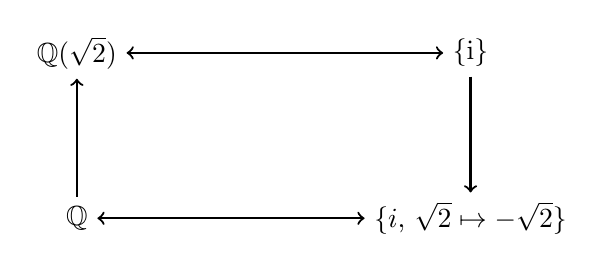
\begin{tikzpicture}
      \node (f) {\(\mathbb{Q}(\sqrt{2})\)};
      \node[below of=f, yshift=-11mm] (e) {\(\mathbb{Q}\)};


      \draw[<-,thick] (f)--(e);

      \node[right of=f, xshift=40mm] (i) {\{i\}};
      \node[below of=i, yshift=-11mm] (h) {\{\(i\), \(\sqrt{2} \mapsto -\sqrt{2}\)\}};


      \draw[->, thick] (i)--(h);


      \draw[<->, thick] (f)--(i);
      \draw[<->, thick] (e)--(h);
    \end{tikzpicture}
    \caption{\footnotesize Field containing \(\sqrt{2}\)}
    \end{figure}

    After the Fundamental theorem, next concept in Galois theory we are applying is the \textbf{Galois field}. The Galois field with GF\((q)\) is a field containing \(q\) number of elements. Since a Galois field contains a finite number of elements it can be represented using finite number of integers \cite{galois} and Galois fields are the finite extension of prime fields.
    \begin{equation*}
      GF(p^n)=\{0,1,...,p-1\} \cup \{p,p+1,...,p+p-1\} \cup ... \cup \{p^{n-1},p^{n-1}+1,...,p^{n-1}+p^{n-2}+...+p-1\}
    \end{equation*}
    where \(p\) is a prime. This representation of a Galois field is called the integer representation. Then\\
    \(GF(2)=\{0,1\}\)\\
    \(GF(2^3)=\{0,1\} \cup \{2,2+1\} \cup \{2^2,2^2+1,2^2+2,2^2+2+1\}=\{0,1,2,3,4,5,6,7\}\)\\

Here, the digits \(2,3,..,7\) of the field \(GF(2^3)\) do not lie in the field \(GF(2)\). If we look the field \(GF(2^3)\) as an extension field of \(GF(2)\) and write its elements using only the elements of the base field \(GF(2)\) then we have the following representations:
\begin{table}[h!]
  \centering
\begin{tabular}{|c|c|c|}
    \hline
    Digits & Expansion & Binary rep..\\
    \hline
    3 & \(2+1\) & 011 \\
    4 & \(2^2+2^1 \times 0 +2^0 \times 0\) & 100 \\
    5 & \(2^2+1\) & 110 \\
    \hline
\end{tabular}
\caption{\small This is actually binary representation of the finite field over GF(2).}
\end{table}

\noindent
For a field \(F\) and an irreducible polynomial \(f(x) \in F[x]\) the quotient ring \(F[x]/(f(x))\) is a field \cite{galois}. If \(F\) is a finite field and \(f(x) \in F[x]\) is irreducible then \(F[x]/(f(x))\) is a finite field. This field consists of all polynomials modulo \(f(x)\). If \(F=GF(2^3)\) then \(x^8+x^7+...+x+1 \in F[x]\) is irreducible in \(F[x]\). Since \(F\) has \(8\) elements which are modulo \(8\), elements of \(F\) is represented by the elements of the factor ring \(F[x]/(f(x))\) \cite{aes}. In the field \(GF(2^3)\), the number \(5\) has the representation \(2^2+1\). This gives the polynomial representation \(x^2+1=(1,0,1)\)(coefficient of \(x^2\) is \(1\) of \(x\) is \(0\) and of constant is \(1\) ) Now the binary equivalent of \(5\) is \(101\). Since the elements of a Galois field can be represented as polynomials the operations are similar to polynomial operations.


\section{Application to the Galois groups of polynomials}
The Fundamental theorem finds its application directly in determining and computing the Galois group of a polynomial. The Galois group of a polynomial gives insights about the nature of roots of the polynomial and tells us whether the polynomial equation can be solved by radicals or not. The Galois group \(G\) of a polynomial \(f \in K[x]\) is the group \(Aut_K^F\), where \(F\) is a splitting field of \(f\) over \(K\) \cite{hunger}. A minimal field \(F\) where a polynomial \(f \in K[x]\) splits into linear factors and thus contains all roots of \(f(x)\) is called a splitting field of \(f\) over \(K\) \cite{hunger}.\\

\noindent
First we can know the nature of the Galois group \(G\) using the Fundamental theorem. The group of automorphism of \(F\) is given by the permutations of roots of \(f\). Hence \(G\) is a subgroup of the symmetric group \(S_n\) \cite{hunger}. Since the  \(F\) is a splitting field of irreducible \(f\) over \(K\) this field \textbf{\(F\) is a Galois extension} of the field \(K\) if all the roots \(u_1,...,u_n\) of \(f\) are simple roots(i.e if \(f\) is separable over \(K\)) so \(F=K(u_1,...,u_n)\). Now for \(u_i \neq u_j\) there exists an field-homomorphism \( \sigma : K(u_i) \mapsto K(u_j) \) which extends to field-automorphism of \(F\) that fixes \(K\). Thus for each \(u_i \neq u_j\) there exists \(\sigma \in G\) such that \(\sigma(u_i) = u_j\) hence the \(G\) is a transitive subgroup of \(S_n\).

\begin{theorem} \cite{hunger}
  Let \(G\) be a Galois group of a polynomial \(f \in K[x]\). \(G\) is isomorphic to a subgroup of some symmetric group \(S_n\). If \(f\) is separable of degree \(n\), the \(n\) divides \(|G|\) and \(G\) isomorphic to a transitive subgroup of \(S_n\).
\end{theorem}

\noindent
If \(f\) is irreducible over the field of rationals \(\mathbb{Q}\) then \(f\) is separable \cite{hunger}. So first we discuss the Galois group of irreducible polynomials. The only non-trivial transitive subgroup of \(S_2\) is \(S_2\) itself hence the Galois groups of an irreducible quadratic polynomial is \(S_2\). The non-trivial transitive subgroups of \(S_3\) are \(A_3\) and \(S_3\) itself. Hence the Galois group of a irreducible cubic is \(A_3\) or \(S_3\). The technique to compute the Galois group of an irreducible quartic is to first determine its resolvant cubic. The cubic polynomial whose roots are \(\alpha\), \(\beta\), \(\gamma\) where, \(\alpha=u_1u_2+u_3u_4,\) \(\beta=u_1u_3+u_2u_4,\) \(\gamma=u_1u_4+u_2u_3\) and  \(u_1, u_2, u_3, u_4\) are the roots of \(f\), is called the resolvant cubic of \(f\) \cite{hunger}. The resolvant cubic is actually a polynomial over \(K\) \cite{hunger}. If \(V=\{(1),(12)(34),(13)(24),(14)(23)\}\) then, under ``the Galois correspondence the subfield \(K(\alpha, \beta, \gamma)\) corresponds to the normal subgroup \(V \cap G\)'' \cite{hunger} because \(K(\alpha,\beta,\gamma)\) is a splitting field of the resolvant cubic whose Galois group is a subgroup of \(S_3\) and only normal subgroup \(N\) of \(S_4\) with \(|N| \leq 6\) is \(V\). ``Hence \(K(\alpha, \beta, \gamma)\) is Galois over \(K\) and \(Aut_K^{K(\alpha, \beta, \gamma)} = G/(G \cap V)\)'' \cite{hunger}.\\[2mm]
Here \(G \subseteq S_4\) so if \([K(\alpha, \beta, \gamma):K=6\)] then from the statement-(i) of the Fundamental theorem we have \(|G/(G \cap V|= [K(\alpha, \beta, \gamma):K]=6\) this gives the Galois group \(G\) of \(f\) is \(S_4\) itself as \(|V|=4\) and \(|G/(G \cap V|=6\) is possible only if \(|G|=24\). Similarly  \([K(\alpha, \beta, \gamma):K]=3\) the \(G=A_4\) and so on.
\clearpage

\begin{figure}[h]
    \centering
  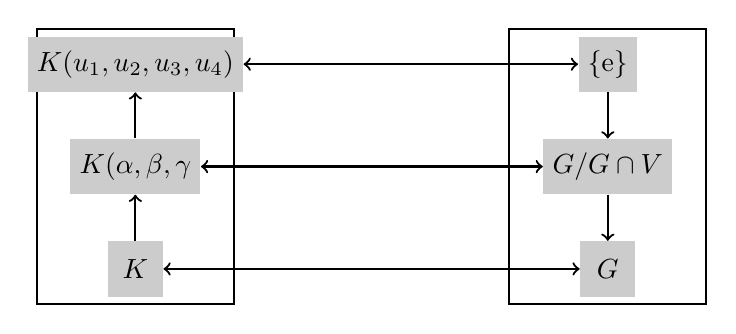
\begin{tikzpicture}

    \node[rectangle, thick, draw,
    minimum height=3.5cm,
    minimum width=2.5cm] (rec) at (0,0) {};

    \node[rectangle, thick, draw,
    minimum height=3.5cm,
    minimum width=2.5cm] (rec2) at (6,0) {};

    \node[minimum width=7mm,
    minimum height=7mm,
    fill=gray!40] (f) at (0,1.3) {\(K(u_1,u_2,u_3,u_4)\)};

      \node[minimum width=7mm,
      minimum height=7mm,
      fill=gray!40,
      below of=f, yshift=-3mm] (e) {\(K(\alpha, \beta, \gamma\)};


      \node[minimum width=7mm,
      minimum height=7mm,
      fill=gray!40,
      below of=e, yshift=-3mm] (k) {\(K\)};

      \draw[<-,thick] (f)--(e);
      \draw[<-,thick] (e)--(k);

      \node[right of=f,
      xshift=5cm,
      minimum width=7mm,
      minimum height=7mm,
      fill=gray!40,
      ] (i) {\{e\}};

      \node[minimum width=7mm,
      minimum height=7mm,
      fill=gray!40,
      below of=i, yshift=-3mm] (h) {\(G/G \cap V\)};

      \node[
      minimum width=7mm,
      minimum height=7mm,
      fill=gray!40,
      below of=h, yshift=-3mm] (g) {\(G\)};

      \draw[->, thick] (i)--(h);
      \draw[->, thick] (h)--(g);

      \draw[<->,thick] (i)--(f);
      \draw[<->,thick] (h)--(e);
      \draw[<->,thick] (g)--(k);
    \end{tikzpicture}
    \caption{\footnotesize Galois correspondence of the quartic}
  \end{figure}

\noindent
The determination and computation of Galois groups of polynomials of degree \(n \geq 5\) is not as easy and straight forward as above because there are no general rules to compute it \cite{hunger}. However we have the following theorem and using this theorem we have computed the Galois groups of two polynomials one of degree \(5\) and another of degree \(7\).

\begin{theorem} \cite{hunger}
  \label{quintic}
If \(p\) is a prime and \(f\) is an irreducible polynomial of degree \(p\) over \(\mathbb{Q}\) which has precisely two nonreal roots, then the Galois group of \(f\) is \(S_p\).
\end{theorem}

\textbf{Galois group of a quintic}\\

\begin{figure}[h!]
  \centering
  \label{quintic-fig}
  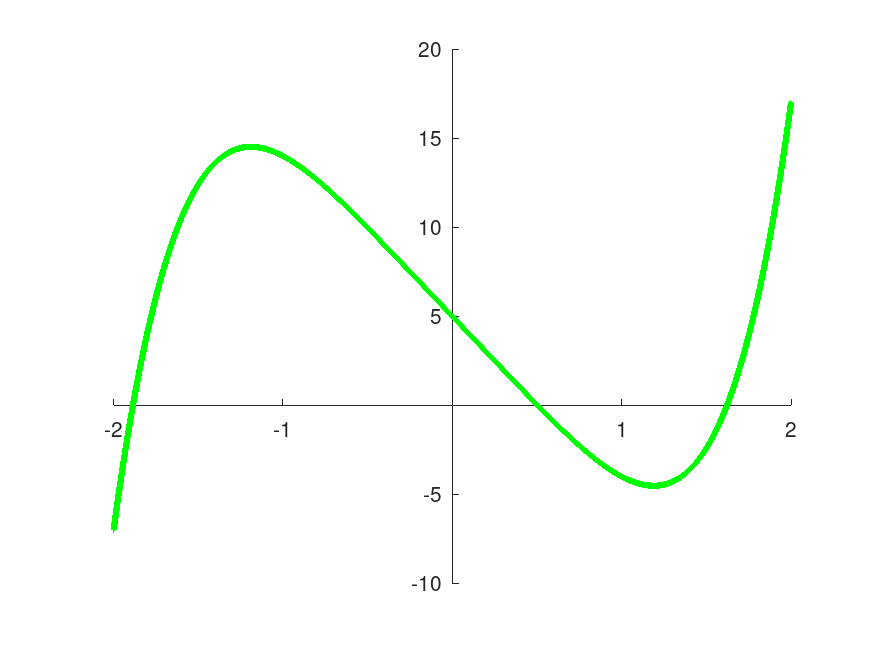
\includegraphics[width=10cm, height=3.2cm]{quantic2.png}
  \caption{\footnotesize Plotted by the ``GNU-Octave'', graph of \(f(x)=x^5-10x+5\) }
\end{figure}
\noindent
The polynomial is \(f(x)=x^5-10x+5 \in \mathbb{Q}[x]\). Its graph is shown above.  From its graph this polynomial has only three real roots. This polynomial is ``irreducible over \(\mathbb{Q}\) by the Eisenstein's criterion'' \cite{hunger} so by Theorem-{\ref{quintic}} its Galois group is \(S_5\) which contains \(5!=120\) elements.\\

\noindent
\textbf{Galois group of a seventh degree polynomial}\\
The polynomial is \(f(x)=x^7-2x^5-4x^3+2x^2+4x-2\) which is ``irreducible over \(\mathbb{Q}\) by the Eisenstein's criterion'' \cite{hunger}. Its graph is shown below.

\begin{figure}[h!]
  \centering
  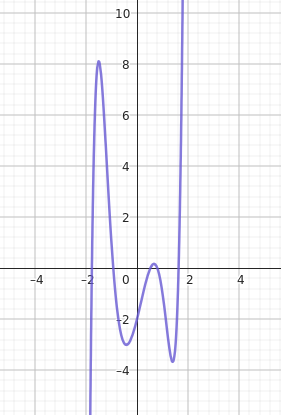
\includegraphics[width=10cm, height=5cm]{seventh2.png}
  \caption{\footnotesize Plotted by the ``Geogebra'', graph of \(f(x)=x^7-2x^5-4x^3+2x^2+4x-2\)}
\end{figure}

\noindent
The graph shows this polynomial has exactly five real roots. So exactly two of its roots are complex. Hence by the Theorem-\ref{quintic} its Galois group is \(S_7\) which contains \(7!=5040\) elements. \\[4mm]

\noindent
The Galois group of a \textbf{reducible polynomial} is computed by factoring it into irreducibles. For an reducible polynomial \(f \in K[x]\), we factor \(f\) into irreducibles as \(f_1f_2...f_k\) and compute the Galois group \(G_i\)  of \(f_i\) for each \(i=1,2,...,k\). Then the Galois group \(G\) of \(f\) is isomorphic to a subgroup of \(\prod G_i\) \cite{algorithm}.

\begin{example}
  The polynomial is \(f(x) = x^4-7x^2+15\)\\
  Here, \(f(x)=(x^2-3)(x^2-5)\) so it is reducible over \(\mathbb{Q}\). Let \(f_1(x)=(x^2-3)\) and \(f_2(x)=(x^2-5)\). Then \(f_1,f_2\) are both irreducible over \(\mathbb{Q}\). The splitting field for \(f_1\) is \(\mathbb{Q}(\sqrt{3})\) so its ``Galois group is \({\mathbb{Z}}_2\)'' \cite{hunger}. The splitting field for \(f_2\) is \(\mathbb{Q}(\sqrt{5})\) so its Galois group is also \({\mathbb{Z}}_2\). Now we have the Galois group of \(f\) is a subgroup of \(G={\mathbb{Z}}_2 \times {\mathbb{Z}}_2\). Since the intersection of \(\mathbb{Q}(\sqrt{3})\) and \(\mathbb{Q}(\sqrt{5})\) is trivial the Galois group of \(f\) is \(G\) itself.
\end{example}

\begin{example}
  The polynomial is \(f(x)=x^7-5x^5-10x^3+5x^2+50x-25 \in \mathbb{Q}[x]\). This polynomial factors into irreducibles over \(\mathbb{Q}\) as \((x^2-5)(x^5-10x+5)\). The Galois group of \(x^2-5\) is \({\mathbb{Z}}_2\) \cite{algorithm} and of \(x^5-10x+5\) is \(S_5\) from above. Also the roots of \(x^2-5\) are \(\sqrt{5}\) and \(-\sqrt{5}\) which are not the roots of \(x^5-10x+5\) from the its graph, Figure-\ref{quintic-fig}. So the intersection of the splitting fields of these two factor polynomials of \(f\) is trivial. Hence the Galois group of \(f\) is \(\mathbb{Z}_2 \times S_5\).
\end{example}

\vspace{5mm}
\noindent
Next we generalize the Galois group of a polynomial in single variable to the \textbf{Galois group of a multi-variable polynomial}. The polynomial is \(f(x,y)=x+y \in \mathbb{Q}[x,y]\). Now the roots of \(f\) over all the complex numbers. Hence its Galois group is \(S_{|\mathbb{C}|}\).
\begin{example}
  The polynomials in \(\mathbb{Q}[x,y]\) are:
  \begin{align}
    y &= x^2+1 \\
    y &=x
  \end{align}
  The roots of these simultaneous polynomials are \(\omega, {\omega}^2\). Then the splitting field of this system is \(\mathbb{Q}(\omega)\). Here the automorphisms of \(\mathbb{Q}(\omega)\) are \(\omega \longmapsto \omega\) and \(\omega \longmapsto {\omega}^2\). Hence the Galois group of this system is \(S_2 \cong {\mathbb{Z}}_2\).
\end{example}

\subsection{Application to the classic problem}
Now we apply the Galois theory to solve the ``classic problem'' using the Galois groups discussed above.  The classic problem is that is every polynomial equation solvable by the method of radicals? Equivalently, does there exist an explicit "formula" which gives all solutions of a polynomial equation? \\If the degree of  the polynomial \(f\) is at most four then the answer is \textbf{yes} \cite{hunger}.\\

\noindent
To answer the above question first we \textbf{formulate} the classic problem into a problem of field theory. The formula by the method of radicals means the formula involving only field operations and the extraction of \(nth\) roots \cite{hunger}. The existence of a formula means there is a finite sequence of steps, each step being a field operation or the extraction of an \(nth\) roots, which yields all solutions of the given polynomial. Performing a field operation leaves the base field unchanged, but the extraction of an \(nth\) root of an element
\(c\) in a field \(K\) amounts to constructing an extension field \(K(u)\) with \(u^n \in K\). Thus the existence of a formula for solving \(f(x)=0\) would imply the existence of a finite tower of fields
\[K=E_0 \subset E_1 \subset ... \subset E_n\]
such that \(E_n\) contains a splitting field of \(f\) over \(K\) and for each \(i \geq 1\), \(E_i=E_{i-1}(u_i)\) with some positive power of \(u_i\) lying in \(E_{i-1}\) \cite{hunger}. An extension field \(F=K(u_1,...,u_n\) of \(K\) such that some power of \(u_1\) lies in \(K\) and for each \(i \geq 2\) some power of \(u_i\) lies in \(K(u_1,...,u_{i-1})\) is called a \textbf{radical extension} of \(K\) \cite{hunger}. Thus the polynomial equation \(f(x)=0\) in rationals is \textit{solvable by radicals} if there exists a radical extension \(F\) of \(K\) and splitting field \(E\) of \(f\) over \(K\) such that \(F \supset E \supset K\). \\[2mm]
Conversely suppose there exists such a tower of fields and that \(E_n\) contains a splitting field of \(f\). Then
\[E_n = K(u_1,u_2,...,u_n)\]
and each solution is of the form \(f(u_1,...,u_n)/g(u_1,...,u_n)\) where \(f,g \in K[x_1,...,x_n]\). Thus each solution is expressible in terms of a finite number of elements of \(K\), a finite number of field operations and \(u_1,...,u_n\). But this amounts to saying that there is a formula for the solutions of the particular given equation \cite{hunger}.

Now that we made a formulation our problem we make a use of the following theorems to deduce the result. The following theorems make a use of group theory which was stated earlier in the Fundamental theorem of Galois theory. A group \(G\) is \textit{solvable} if it has a solvable series and a finite chain of subgroups \(G=G_0>G_1>...>G_n={e}\) such that \(G_{i+1}\) is normal in \(G_i\) for \(0 \leq i < n\) and  each factor group \(G_i/G_{i+1}\) is abelian is called a \textit{solvable series}.
\begin{theorem} \cite{hunger}
  \begin{enumerate}
  \item If \(F\) is a radical extension of \(K\) and \(E\) is an intermediate field, then \(Aut_K^E\) is a solvable group
    \item If the polynomial equation \(f(x)=0\) in rationals is solvable by radicals, then the Galois group of \(f\) is a solvable group.
    \item The symmetric group \(S_n\) is not solvable for \(n \geq 5\).
      \end{enumerate}
\end{theorem}

\noindent
The polynomial \(f(x)=x^5-10x+5 \in \mathbb{Q}[x]\) has Galois group ``\(S_5\), which is not a solvable group'' \cite{hunger}. The quintic polynomial equations over \(\mathbb{Q}\) are not solvable by radicals. That is there does not exist an explicit formula for solving the quintics. Moreover, ``polynomial equations of degree \(n \geq 5\) are not solvable by radicals'' \cite{hunger}.\\[2mm]

\noindent
Galois theory gives the precise condition under which a polynomial of degree \(n \geq 5\) is solvable by radicals or not.
\begin{example}
  The polynomial is \(x^5-1 \in \mathbb{Q}[x]\).\\
  The set of  roots of this polynomial are the fifth roots of unity which forms a group under addition modulo \(5\). Hence the ``Galois group is isomorphic to \(\mathbb{Z}_5\)'' \cite{hunger}. The group \(\mathbb{Z}_5\) is cyclic and ``every cyclic group is solvable'' \cite{galois}. Hence this polynomial can be  solved by radicals.
\end{example}

\section{Application to the Coding theory}
The Galois fields are applied in coding theory in computer science. The loss of information is inevitable. It cannot be prevented or stopped. So, we need a way of retrieving the lost information or correcting the false information.

\begin{enumerate}
\item Paintings gets deteriorated over time and has to be renovated.
\item The data stored in a CD is lost over time \cite{coding}.
\end{enumerate}

\noindent
To be able to detect and correct errors during transmission of information in digital system coding theory is developed. In digital system, information are transmitted as strings of \(0\) and \(1\). So the fundamental of the coding theory is the manipulation of strings of binary digits. The proper and complete manipulation of these strings is possibly only if the space of the strings is a field. This finite field is a Galois field. The widely used field for coding in electronically transmitting device is an extension field \({\mathbb{Z}}_2\) which is the field \(GF(2)\) consisting of \(0\) and \(1\). Recent works has shown that it is possible to extend codes to more general type of numbers called rings. This rings are called "Galois rings" \cite{error_correct}. The idea of coding theory is to append some extra digits to the information and use this to detect and possibly correct the errors during transmission. These codes are called error-correcting codes \cite{coding}. One of such error-correcting code is a linear code which is a linear space.

\begin{definition} \cite{error_correct} [\textbf{Linear code}]
  \label{linear}
Let \(K=GF(q)\) be a Galois field. Then a finite extension of \(K\) of dimension \(n\) is \(V=GF(q)^n=GF(q^n)\). A linear code \(C\) is a subspace of \(V\). The code \(C\) has dimension \(k \leq n\) and the length \(n\). It is called a \((n,k)\) code.
\end{definition}

\noindent
The usefulness of linear code is that they are vector spaces over the base field so they have a basis. All the code words can be generated with this basis. Instead of storing all \(2^k\) number of code words (for \(k\)-dimensional binary codes), storing only \(k\) basis elements is sufficient which saves massive storage. For the code \(C\) the generator matrix is defined as follows:

\begin{definition} \cite{error_correct} [\textbf{Generator Matrix}]
  Let \(\{v_1, v_2,...,v_k\}\) be a basis of \(C\). A generator matrix is the \(k \times n\) matrix \(G=\begin{pmatrix} \small
      v_1\\
      v_2\\
      ...\\
      v_k
    \end{pmatrix}
  \).
\end{definition}

\noindent
The dual code of \(C\) is the set \(C^{\perp}=\{x \in V \;| \; x.y=0 \;\; \forall y \in V \}\) \cite{error_correct}. The dual code is a code in itself and has dimension \(n-k\). The \(C^{\perp}\) is linear so it has a generator matrix.A generator matrix \(H\) of \(C^{\perp}\) is called a \textbf{parity check matrix}. To apply \((n,k)\) coding first we need to group our information into the blocks of length \(k\). \(u_1,...,u_k\),  \(u_k,...,u_{2k}\),... . This space has dimension \(k\). Now these block of codes are encoded separately each to a code of length \(n\) as shown \cite{coding}.

\vspace{5mm}
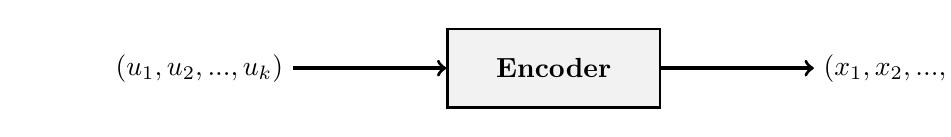
\begin{tikzpicture}
  \hspace{1cm}
  \node [] (u) {\((u_1,u_2,...,u_k\))};
  \node[
  right of=u,
  rectangle,
  draw,
  thick,
  fill=gray!10,
  minimum width=27mm,
  minimum height=10mm,
  xshift=35mm] (e) {\bfseries Encoder};

  \node[right of=e, xshift=35mm] (x) {\((x_1,x_2,...,x_n)\)};

  \draw[->,very thick] (u)--(e);
  \draw[->,very thick] (e)--(x);
\end{tikzpicture}

\noindent
Mathematically, the encoded vector \(x\) is obtained form the original vector \(u\) using the generator matrix \(G\) by the relation \(x=uG\) \cite{coding}.\\[3mm] To continue and complete the diagram.\\

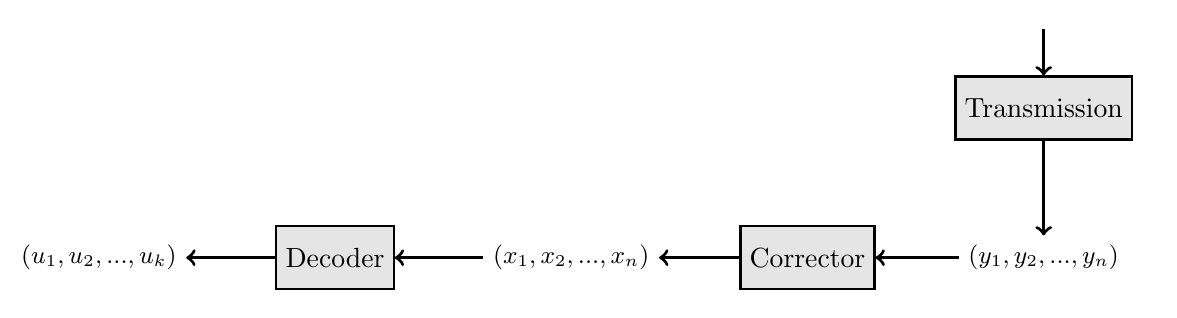
\begin{tikzpicture}
  \hspace{-2mm}
  \node[
  rectangle,
  draw,
  thick,
  fill=gray!20,
  minimum width=13mm,
  minimum height=8mm,
  ] (t) {Transmission};

  \node[below of=t, yshift=-9mm] (y) {\small \((y_1,y_2,...,y_n\))};

  \node[
  left of=y,
  rectangle,
  draw,
  thick,
  fill=gray!20,
  minimum width=13mm,
  minimum height=8mm,
  xshift=-20mm] (c) {Corrector};

  \node[left of=c, xshift=-20mm] (x) {\small \((x_1,x_2,...,x_n)\)};

  \node[
  left of=x,
  rectangle,
  draw,
  thick,
  fill=gray!20,
  minimum width=13mm,
  minimum height=8mm,
  xshift=-20mm] (d) {Decoder};

  \node[left of=d, xshift=-20mm] (u) {\small \((u_1,u_2,...,u_k\))};


  \draw[->,very thick] (0,1)--(t);
  \draw[->,very thick] (t)--(y);
  \draw[->,very thick] (y)--(c);
  \draw[->,very thick] (c)--(x);
  \draw[->,very thick] (x)--(d);
  \draw[->,very thick] (d)--(u);
\end{tikzpicture}

\vspace{2mm}
\noindent
We have a way of correcting the received information if it is distorted. This way of correcting is called \textbf{Syndrome correcting} because it makes use of the syndrome of the received vector which is defined as follows:
\begin{definition} \cite{error_correct} [\textbf{Syndrome}]
  The syndrome of a vector \(y \in V\) is defined as \\ \(syn(y)=\begin{pmatrix} \small
    y.h_1\\
    y.h_2\\
    ...\\
    y.h_{n-k}
  \end{pmatrix}\), \hspace{12mm} where
  \(\begin{pmatrix}
    h_1 \\ h_2\\ ...\\ h_{n-k}
  \end{pmatrix}\) is the parity check matrix of \(C\).
\end{definition}
\noindent
Now the code \(C\) is a subgroup of \(V\) under addition moreover it is a normal subgroup of \(V\). Two vectors in \(V\) have the same syndrome if and only if they are in the same co-set of \(C\) \cite{error_correct}. Then we have the following correcting process. Suppose the signal received is the vector \(y\).
\begin{enumerate}
\item First we determine its syndrome, \(syn(y)\).
\item Determine the co-set of \(C\) containing \(syn(y)\), say \(e + C\).
\item Then \(y=e+x\) for some \(x \in C\). This implies \(x=y-e\). Since \(x \in C\), this \(x\) is the required correction of \(y\) \cite{error_correct}.
\end{enumerate}
This \(e\) is also called "error vector" \cite{error_correct}.

\begin{example}
  Consider a generator matrix \( \small G=\begin{pmatrix}
    1 & 0 & 1 & 0\\
    0 & 1 & 1 & 1
  \end{pmatrix}\). Then the parity check matrix is \(H=\begin{pmatrix}
    1 & 1 & 1 & 0\\
    0 & 1 & 0 & 1
  \end{pmatrix}\). And the code generated by \(G\) is \\ \(C=\{(0,0,0,0),(1,0,1,0),(0,1,1,1),(1,0,1,1)\} \;\; \subset GF(2^{4})\).\\

  Suppose the received vector is \(y=(1,1,1,0)\). Then \(y \not \in C\) so the information is distorted from the original information. To get the original information:\\
  \(syn(y)= \begin{pmatrix}
    y.h_1 \\ y.h_2
  \end{pmatrix} = \begin{pmatrix}
    1 \\ 1
  \end{pmatrix}\) where \(h_1\) is the first row and \(h_2\) is the second row of \(H\).\\
  Now if \(e=(0,1,0,0)\) then \(e+C=\begin{pmatrix}
    1 \\ 1
  \end{pmatrix}\) so \(y-e=(1,1,1,0)-(0,1,0,0)=(1,0,1,0) \in C\) is the original information \cite{error_correct}.
\end{example}

\noindent
There is a more sophisticated error-correcting code than the linear codes called the \textbf{cyclic code}. Linear codes are simple to implement but the correcting algorithm of linear codes are not efficient as it makes use of matrix which is the generating matrix. The code \(C\) as defined in \ref{linear} is cyclic if \((a_0,a_1,...,a_{n-1}) \in C \implies (a_{n-1},a_0,...,a_{n-2}) \in C\). Suppose \(C\) is a code over a Galois field \(F=GF(q)\). Then there exist a correspondence \(\Phi : C \mapsto F[x]/(x^n-1)\) such that \(\{(a_0,a_1,...,a_{n-1}),(a_1,...,a_{n-1},a_0),....,(a_{n-1},a_0,....,a_{n-2})\} \longmapsto a_0+a_1x+a_2x^2+...+a_{n-1}x^{n-1}\). This map \(\Phi\) is a homomorphism. This shows that the cyclic code \(C\) can be embedded into the ring \(R_n=F[x]/(x^n-1)\) \cite{error_correct}. For this reason cyclic codes are represented using polynomial representation. We have the following theorem that characterizes the cyclic code.

\begin{theorem} \cite{error_correct}
A subset \(S\) of \(R_n\) corresponds to a cyclic code if and only if \(S\) is an ideal of \(R_n\) and if \(S=(g(x))\) if and only if  \(g(x)\) divides \(x^n-1\).
\end{theorem}

\noindent
This theorem determines all cyclic codes of a Galois field \(GF(p^n)\). They are ideals of \(R_n\) and these ideals are generated by the polynomials that divides \(x^n-1\). Thus cyclic codes have a generator polynomial which is computationally simpler than having a generator matrix. Due to this some cyclic codes have efficient correcting algorithms.

\begin{example}
  The divisors of \(x^3-1 \in F=GF(2^{3})\) are \(1, x+1, x^2+x+1, x^3-1\).\\
  For \(g(x)=x+1\) we have \(F[x]/(g(x))=\{(0),(1+x),(1+x^2),(x+x^2)\}\) using the binary notation from the polynomial notation we have the corresponding cyclic code is \(\{(0,0,0),(1,1,0),(1,0,1),(0,1,1)\}\) \cite{error_correct}.
\end{example}
Some usages of the error-correcting codes are as follows:
\begin{enumerate}
\item The \((3,1)\) binary code is used in the short-range wireless communication system like \(Bluetooth^{TM}\) \cite{wireless}.
\item The Hamming Code \((7,4)\) is used in memory devices like RAM \cite{coding}.

\item The Cyclic codes are used in storing data in CDs and DVDs \cite{coding}.
\end{enumerate}


\section{Application to the Cryptography}
\noindent
Cryptography is the science of safe-guarding information by converting the original message into something different. Galois fields are the life of modern cryptography used in digital communication. Advance Encryption Standard(AES) is one of the widely used cryptography standard developed by two Belgian cryptographers,  \textit{Vincent Rijmen and Joan Daemen} \cite{aes} which make a use of Galois field. The AES is a computer security standard for cryptography which is approved by the ``Federal Information Processing Standards Publications'' of USA which became effective on May 26, 2002. ``The AES algorithm is a \textit{symmetric block cipher} that can encrypt and decrypt digital information'' \cite{aes}. Symmetric key cryptography is used to share information between two parties where the two parties share a secret ``key'' and a public encryption algorithm \cite{wireless}. The generic algorithm of AES consists of smaller sub-algorithms namely ``Sub-Bytes, Shift-Rows, Mix-Columns and Add-Round-Key'' \cite{aes}.\\[2mm]

\noindent
\textbf{The State}\\[1mm]
First the data is broken into blocks and each block is broken into smaller chunks of a size byte (16 bytes for a block of size 128bits). This block is then represented in a  which consisting of bytes of the word. This matrix is called the State. Mathematical operations are not applicable to the data directly so the significance of this step is to make the data applicable for mathematical operations. For the 128-bit key encryption the algorithm forms a \(4 \times 4\) matrix with each entry of a size one byte. This matrix can afford to evaluate a data of size 16 byte at a time \cite{aes}.\\[2mm]

\noindent
\textbf{Sub-Bytes}\\[1mm]
In this step, first each byte of the matrix is replaced with its multiplicative inverse if it has one. Then it transforms each bytes using an invertible affine transformation, \(x \mapsto Ax+b\) \cite{aes}.\\[2mm]

\noindent
\textbf{Mathematical Preliminaries}\\[1mm]
Each byte in the state i.e each entry in the matrix, is interpreted as one of the 256 elements of a finite field \(GF(2^8)\). Then the addition, multiplication operations are performed according to the respective field operations of the field \(GF(2^8)\). \\[2mm]

\noindent
\textbf{Shift-Rows}\\[1mm]
In this step entries of a row is shifted to scramble data. Row-n shifted to the left by \(n-1\) unit. Here,\\
\(1-1=0\), so row-1 is left unchanged. \(2-1=1\), so row-2 is shifted to the left by 1 unit and row-3 by 2 unit and so on as shown below \cite{aes}.

If \(A=\begin{bmatrix}
    a_{11}&a_{12}&a_{13}&a_{14}\\
    a_{21}&a_{22}&a_{23}&a_{24}\\
    a_{31}&a_{32}&a_{33}&a_{34}\\
    a_{41}&a_{42}&a_{43}&a_{44}
    \end{bmatrix}\) \hspace{3mm} then \(A'=\begin{bmatrix}
    a_{11}&a_{12}&a_{13}&a_{14}\\
    a_{22}&a_{23}&a_{24}&a_{21}\\
    a_{33}&a_{34}&a_{31}&a_{32}\\
    a_{44}&a_{41}&a_{42}&a_{43}
  \end{bmatrix}\)  is the matrix after Shit-Row.\\[2mm]

\noindent
\textbf{Mix-Columns} \\[1mm]
In this step each column is transformed using a linear transformation, \(c \mapsto Bc\) where \(c\) is a column of the matrix obtained above. Since linear transformation is invertible this step is invertible. Note every step of this algorithm must be invertible to be able to decrypt the data \cite{aes}. \\[2mm]

\noindent
\textbf{Add-Round-Key} \\[1mm]
This is the step where the encrypted data gets uniqueness. Each user is assigned an "unique key" and this key is added to the matrix obtained from the last step \cite{aes}.\\[3mm]

\noindent
\textbf{Illustration}\\
Let us encrypt the sentence "Fun Cryptography". This consists of exactly 16 characters.
\begin{enumerate}
\item First we write the ASCII representation of each character of the sentence as shown below. We do so because the ASCII representation gives the binary representation of each character which has a size of a byte. The ASCII representation of "F" is \(70\) which is \(01000110\) in binary.
  \[\begin{bmatrix}
      70 & 117 & 110 & 32 \\
      67 & 114 & 121 & 112\\
      116 & 111 & 103 & 114 \\
      97 & 112 & 104 & 121
    \end{bmatrix}=
    \begin{bmatrix}
      01000110 & 01110110 & 01101110 & 00010000 \\
      01000011 & 01110010 & 01111001 & 01110000\\
      01110100 & 01101111 & 01100111 & 01110010 \\
      01100001 & 01110000 & 01101000 & 01111001
    \end{bmatrix}
  \]


\item After performing Sub-Bytes, Shift-Rows, Mix-Columns, we get the following matrix.

  \[\begin{bmatrix}
      11100111 & 00011000 & 00100100 & 01110000\\
      00101010 & 10101011 & 00111001 & 01100011\\
      00010101 & 01100101 & 11110111 & 10100111\\
      10101011 & 11110110 & 00000011 & 10100100
    \end{bmatrix}=
    \begin{bmatrix}
      231 & 24 & 36 & 112\\
      42 & 171 & 57 & 99\\
      21 & 101 & 247 & 167\\
      171 & 246 & 3 & 164
    \end{bmatrix}
  \]

\item We have omitted the Add-Round-Key step just for the sake of simplicity. The matrix obtained at last in step-2 translates to something different from our original sentence.

\item The decryption process is applying the inverse of the encryption process \cite{aes}.
\end{enumerate}

% -------------------------------------------------------------------------------------------
\vspace{5mm}
\textbf{Conclusions}\\
The Galois theory that begun in the 19th century due to the french mathematician \textit{Évariste Galois} is still a relevant field of research today. Over the 200 years this theory has found its development as a linking theory of the two main theories: Group theory and field theory. It has found its applications in both pure and applied mathematics; where-ever ``Field Theory'' has anything to do with.\\
Many concepts of Abstract algebra, Algebraic number theory, Algebraic geometry, etc rely heavily on Galois theory because they are developed on field extensions, and the computer science relies heavily on Galois field.\\

\textbf{Acknowledgment:} \\
I would like to thank \textit{Kathmandu Center for Research and Education Chinese Academy of Sciences-TU} for awarding me with
\textit{KCRE Excellent Student Thesis Grant 2023(Grant number: 08092023)}\\ to financially aid me for this research.
\vspace{7mm}


% --------------------------------------------------------------------------------------------------------------------------------------------------

\begin{thebibliography}{9}
\bibitem{galois}
Escofier, J. P. (2000) \emph{Galois Theory}. Springer, New York.

\bibitem{error_correct}
Holdman, G. R. (2019) \emph{Error Correcting Codes  Over Galois Rings}. Graduate Dissertation, Department of Mathematics, Whitman college, 345 Boyer Ave.
Walla Walla, Washington, U.S.A.

\bibitem{hunger}
Hungerford, T. W. (2012) \emph{Algebra}. Springer (India), New Dheli.

\bibitem{algorithm}
Lenstra, A., Lenstra, H.,  \& Lovasz, L. (1982)  Factoring polynomials with rational coefficients. \emph{Mathematische Annalen},261,12.

\bibitem{coding}
Neubaer, A.,  Freudenberger, J.,  \& Kuhn, V. (2007) \emph{Coding Theory, Algorithms, Architectures, and Applications}. John Wiley and Sons Ltd, Chichester, West Sussex, England:1-93.

\bibitem{wireless}
Sarma, D. (2018) Implementation of Galois Field for Application in Wireless Communication Channels. \emph{MATEC Web of Conferences},2010:03012.

\bibitem{aes}
National Institute of Standards and Technology. (2001) Advanced Encryption
Standard (AES). \emph{(Department of Commerce, Washington, D.C.), Federal Information Processing Standards Publication (FIPS) NIST FIPS}. 197-upd.1 updated May 9, 2023. doi:10.6028/NIST.FIPS.197-upd1.

\end{thebibliography}
\end{document}

%%% Local Variables:
%%% mode: latex
%%% TeX-master: t
%%% End:
